\documentclass{beamer}
% \documentclass[handout]{beamer}

% Settings and commands
\usepackage[utf8]{inputenc} % Accept different input encodings
\usepackage{mathtools} % Extra symbols and fixes to amsmath
\usepackage{thmtools} % Theorem tools
\usepackage{graphicx}
% \usepackage[shortlabels]{enumitem} % Customising lists - incompatible with beamer
\usepackage{centernot} % Centred negation slash
\usepackage{hyperref}
\usepackage{tcolorbox} % Boxes surrounding text
\usepackage{tikz-cd} % Commutative diagrams
\usepackage{newtx} % Nicer font
\usepackage{bookmark} % Hyperlinks and bookmarks
\usepackage{xcolor}
\usepackage{tkz-base}
\usepackage{tkz-graph}
\usepackage{tkz-euclide}
\usepackage{tikzscale}
\usepackage{listings}
\usepackage{csquotes}
\usepackage{accsupp}
\newcommand{\emptyaccsupp}[1]{\BeginAccSupp{ActualText={}}#1\EndAccSupp{}}

\usetheme[progressbar=frametitle]{metropolis}
\usefonttheme{professionalfonts}
\newcounter{insub}
\AtBeginSubsection[]{\setcounter{insub}{0}}
\AtBeginEnvironment{slide}{\addtocounter{insub}{1}}
\newenvironment<>{slide}{\begin{frame}#1%
        \frametitle{\subsecname{}\ifthenelse{\theinsub=1}{}{\enskip(\roman{insub})}}
        }{\end{frame}}
% \setbeamertemplate{theorems}[numbered]
\definecolor{metropolis}{HTML}{FAFAFA}

% ---------------------------------------- %
% SETTINGS

\tcbuselibrary{breakable}
\newtcolorbox{framedbox}{standard jigsaw, opacityback=0, boxrule=1pt, breakable, before skip=8pt, after skip=8pt}

% \let \originalLeft \left % Fixing \left and \right
% \let \originalRight \right
% \renewcommand{\left}{\mathopen{} \mathclose \bgroup \originalLeft}
% \renewcommand{\right}{\aftergroup \egroup \originalRight}

\newtheorem{proposition}{Proposition}

%% tkz-graph
% \GraphInit[vstyle=Hasse]
% \GraphInit[vstyle=Welsh]
% \GraphInit[vstyle=Normal]
% \GraphInit[vstyle=Classic]
\SetGraphUnit{1}
\SetVertexMath
\tikzset{VertexStyle/.append style={minimum size=8pt}}

%% listings
% Code block styles (listings)
\definecolor{codegreen}{rgb}{0,0.6,0}
\definecolor{codegray}{rgb}{0.5,0.5,0.5}
\definecolor{codepurple}{rgb}{0.58,0,0.82}
\definecolor{backcolour}{rgb}{0.95,0.95,0.92}
\lstdefinestyle{default}{
    basewidth={.5em,0.5em},
    basicstyle=\ttfamily,
    breakatwhitespace=false,
    breaklines=true,
    captionpos=b,
    xleftmargin=15pt,
    framexleftmargin=2pt,
    framexrightmargin=2pt,
    keepspaces=true,
    numbers=left,
    numbersep=5pt,
    tabsize=4,
    columns=fullflexible,
    backgroundcolor=\color{backcolour},
    commentstyle=\itshape\color{codegreen},
    keywordstyle=\color{magenta},
    numberstyle=\footnotesize\itshape\color{black}\emptyaccsupp,
    stringstyle=\color{codepurple}
}
% \lstdefinelanguage{GAP}{%
%     morekeywords={%
%             Assert,Info,IsBound,QUIT,%
%             TryNextMethod,Unbind,and,break,%
%             continue,do,elif,%
%             else,end,false,fi,for,%
%             function,if,in,local,%
%             mod,not,od,or,%
%             quit,rec,repeat,return,%
%             then,true,until,while%
%         },%
%     sensitive,%
%     morecomment=[l]\#,%
%     morestring=[b]",%
%     morestring=[b]',%
% }[keywords,comments,strings]
\lstset{style=default,language=GAP}
\input{commands.tex}

\title{\textbf{Rubik's cubes and permutation group theory}}
\author{\textbf{Lawrence Chen}}
\institute{\textbf{Honours presentation}}
\date{\today}

\titlegraphic{
\vspace{3.75cm}\flushright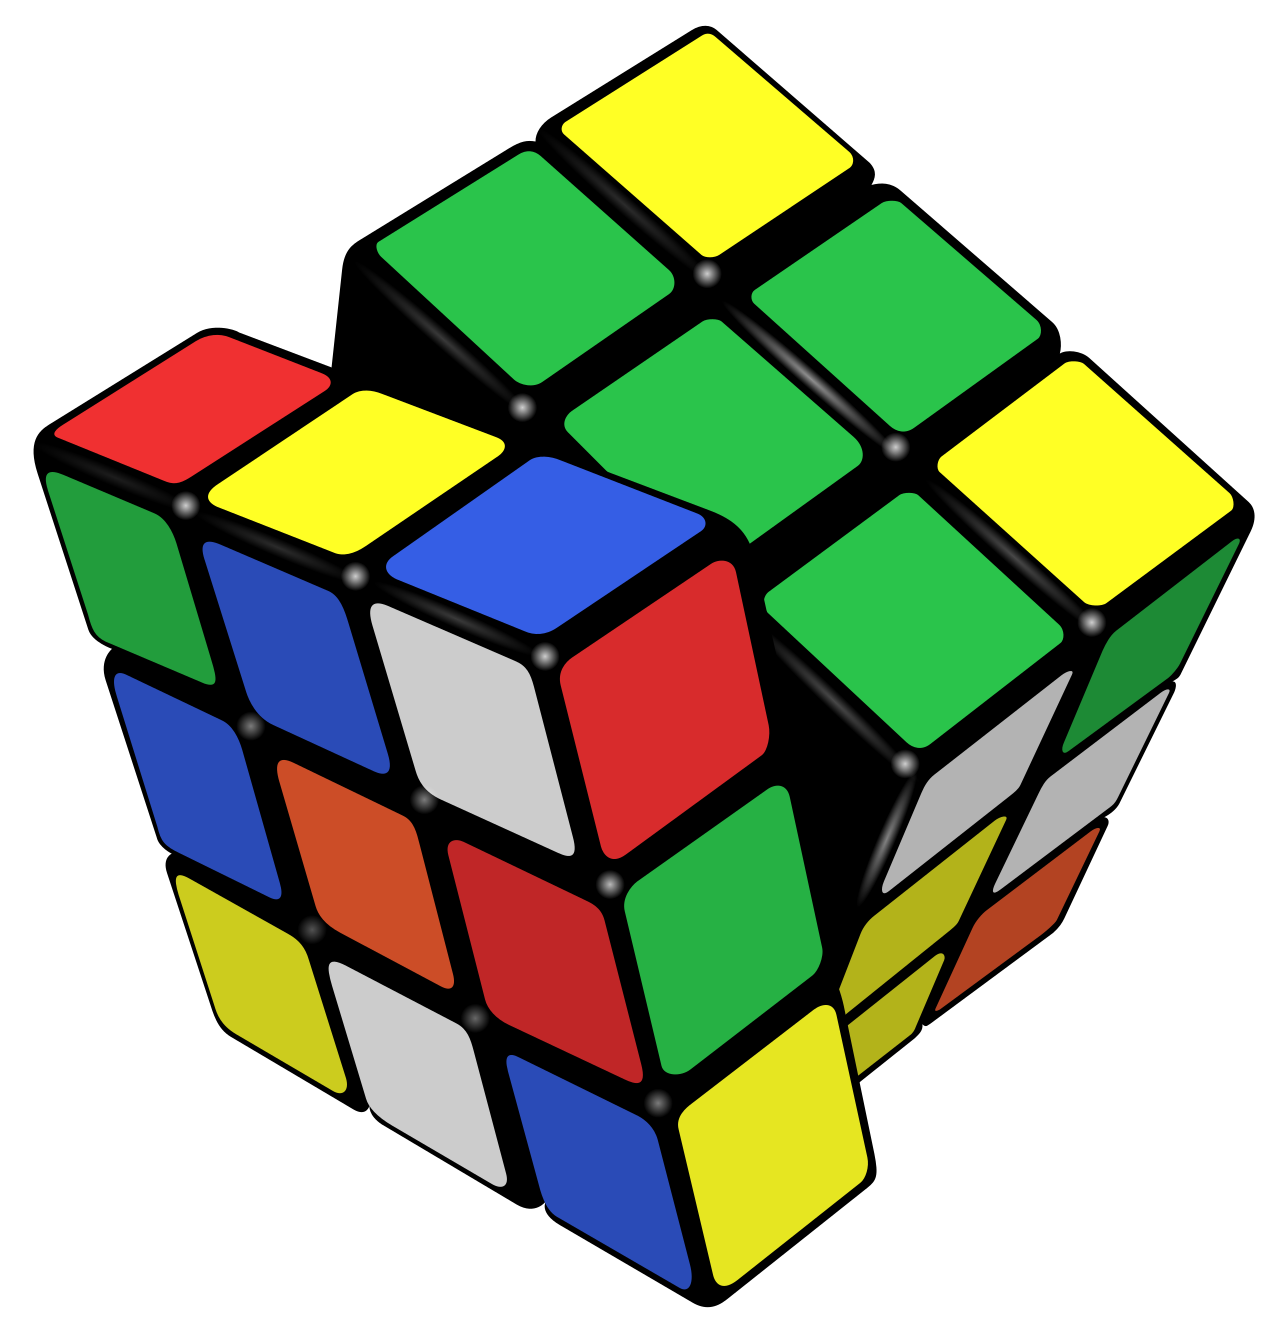
\includegraphics[width=0.4\textwidth]{graphics/rubiks_cube_title.png}
}

\setbeamerfont{subsection in toc}{size=\footnotesize}
\newcommand{\RC}{\mathcal{G}}
\newcommand{\RS}{\mathcal{S}}
% \metroset{block=fill}

\begin{document}

\begin{frame}[plain, noframenumbering]
    \titlepage
\end{frame}

\begin{frame}[plain, noframenumbering]{Contents}
    % \tableofcontents[hideallsubsections]
    \begin{columns}[t]
        \begin{column}{.5\textwidth}
            \tableofcontents[sections={1-2}]
        \end{column}
        \begin{column}{.5\textwidth}
            \tableofcontents[sections={3-4}]
        \end{column}
    \end{columns}
\end{frame}

\subsection{Questions about Rubik's cube}

\begin{slide}
    \begin{itemize}
        \item How can we represent \textit{move sequences} and \textit{states} of a cube? \pause
        \item How can we tell \textit{how many} states a Rubik's cube can take? \pause
        \item If we repeat a move, do we eventually \textit{get back to the start}? \pause
        \item If a Rubik's cube is \textit{restickered}, is it \textit{solvable}? \pause
        \item How can we use maths to \textit{solve} a Rubik's cube? \pause
    \end{itemize}

    \textit{Answer:} using permutations and \textit{computational group theory}! \pause

    \begin{alertblock}{(J. A. Paulos, Innumeracy)}
        \vspace{4pt}
        \begin{quotation}
            Ideal Toy Company stated on the package of the original Rubik cube that there were more than three billion possible states the cube could attain. It's analogous to McDonald's proudly announcing that they've sold more than 120 hamburgers.
        \end{quotation}
    \end{alertblock}
\end{slide}

\section{Some basic group theory}

\subsection{Permutations}

\begin{slide}
    \begin{definition}[permutation]
        \vspace{0pt}
        \textbf{Permutation} of $[n] := \{1,\dotsc,n\}$ is bijection $\sigma : [n] \to [n]$. \textbf{Symmetric group} $\Sym(n)$ is set of permutations of $[n]$.
    \end{definition}

    \onslide<2->{Write $1 = ()$ for identity. Write $i^\sigma$ not $\sigma(i)$ for \textit{image}.

        \onslide<3->{\textit{Cycle notation:} $\sigma = (1,4,5)(2,6) \in \Sym(6)$ is:

            \begin{center}
                \begin{tikzpicture}[x=1cm,y=2cm]
                    \GraphInit[vstyle=Normal]
                    \tikzset{VertexStyle/.style={draw=none}}
                    \tikzset{EdgeStyle/.style={->}}
                    \Vertex{1} \EA(1){2} \EA(2){3} \EA(3){4} \EA(4){5} \EA(5){6}
                    \SO[L=1](1){1'} \SO[L=2](2){2'} \SO[L=3](3){3'} \SO[L=4](4){4'} \SO[L=5](5){5'} \SO[L=6](6){6'}
                    \onslide<4->{\Edge(1.south)(4'.north)}
                    \onslide<5->{\Edge(4.south)(5'.north)}
                    \onslide<6->{\Edge(5.south)(1'.north)}
                    \onslide<7->{\Edge(2.south)(6'.north)}
                    \onslide<8->{\Edge(6.south)(2'.north)}
                    \onslide<9->{\Edge(3.south)(3'.north)}
                    \tkzDefPoint(-0.5,-0.5){lab}\tkzLabelPoint[left](lab){$\sigma$}
                \end{tikzpicture}
            \end{center}

            It means
            $$\onslide<4->{1^\sigma = 4,\ \onslide<5->{4^\sigma = 5,\ \onslide<6->{5^\sigma = 1,\ \onslide<7->{2^\sigma = 6,\ \onslide<8->{6^\sigma = 2,\ \onslide<9->{3^\sigma = 3.}}}}}}$$}}
\end{slide}

\begin{slide}
    \textit{Product/composition:} for $\sigma,\tau \in \Sym(n)$, $\sigma\tau$ means ``first $\sigma$, then $\tau$'', so $i^{\sigma\tau} = (i^\sigma)^\tau$. \onslide<2->{E.g. $\sigma = (1,2,3),\onslide<3->{\tau = (1,3)(2,4) \in \Sym(4)$,}

    \begin{center}
        \begin{tikzpicture}[x=1cm,y=1.5cm]
            \GraphInit[vstyle=Normal]
            \tikzset{VertexStyle/.style={draw=none}}
            \tikzset{EdgeStyle/.style={->}}
            \Vertex{1} \EA(1){2} \EA(2){3} \EA(3){4}
            \SO[L=1](1){1'} \SO[L=2](2){2'} \SO[L=3](3){3'} \SO[L=4](4){4'}
            \Edge(1.south)(2'.north) \Edge(2.south)(3'.north) \Edge(3.south)(1'.north) \Edge(4.south)(4'.north)
            \tkzDefPoint(-0.5,-0.5){lab}\tkzLabelPoint[left](lab){$\sigma$}
            \onslide<3->{\SO[L=1](1'){1''} \SO[L=2](2'){2''} \SO[L=3](3'){3''} \SO[L=4](4'){4''}
                \Edge(1'.south)(3''.north) \Edge(3'.south)(1''.north) \Edge(2'.south)(4''.north) \Edge(4'.south)(2''.north)
                \tkzDefPoint(-0.5,-1.5){lab2}\tkzLabelPoint[left](lab2){$\tau$}
            }
            \onslide<4->{
                \EA[unit=3,L=1](4){c1} \EA[L=2](c1){c2} \EA[L=3](c2){c3} \EA[L=4](c3){c4}
                \EA[unit=3,L=1](4''){c1'} \EA[L=2](c1'){c2'} \EA[L=3](c2'){c3'} \EA[L=4](c3'){c4'}
                \onslide<5->{\Edge(c1.south)(c4'.north)}
                \onslide<6->{\Edge(c4.south)(c2'.north)}
                \onslide<7->{\Edge(c2.south)(c1'.north)}
                \onslide<8->{\Edge(c3.south)(c3'.north)}
                \tkzDefPoint(5.5,-1){lab3}\tkzLabelPoint[left](lab3){$\sigma\tau$}
            }
        \end{tikzpicture}
    \end{center}
    \onslide<4->{$$\sigma\tau = (1,2,3)(1,3)(2,4) = (1,\onslide<5->{4,\onslide<6->{2\onslide<7->{)\onslide<8->{\in \Sym(4).}}}}$$}}

    \vspace{-0.5cm}
    \textit{Note:} here, $\sigma\tau \neq \tau\sigma$, since $1^{\sigma\tau} = 4$ but $1^{\tau\sigma} = (1^\tau)^\sigma = 3^\sigma = 1$. Identity $1 = ()$ satisfies $1 \sigma = \sigma 1 = \sigma$ for $\sigma \in \Sym(n)$.
\end{slide}

\subsection{Permutation groups}

\begin{slide}
    \textit{Note:} for $g,h,k \in \Sym(n)$, (i) $gh \in \Sym(n)$, (ii) $1 = () \in \Sym(n)$, (iii) $g^{-1} \in \Sym(n)$, (iv) $(gh)k = g(hk)$. If true for subset:

    \begin{definition}[permutation group]
        \vspace{0pt}
        \textbf{Permutation group} of degree $n$ is subset $G \leq \Sym(n)$ satisfying:
        \begin{enumerate}[(i)]
            \item \textbf{(closure)} $gh \in G$ for $g,h \in G$; \pause
            \item \textbf{(identity)} $1 = () \in G$; \pause
            \item \textbf{(inverses)} $g^{-1} \in G$ for $g \in G$.
        \end{enumerate}
    \end{definition}

    \begin{example}[alternating group]
        \vspace{0pt}
        \textbf{Alternating group} $\Alt(3) = \{(),(1,2,3),(1,3,2)\} < \Sym(3)$. \\
        In general, $\Alt(n)$ is all \textit{even} permutations of $[n]$ (product of even \# of \textit{transpositions} $(i,j)$, e.g. $(1,2,3) = (1,2)(1,3)$).
    \end{example}
\end{slide}

% \subsection{Order of permutations}

% \begin{slide}
%     \begin{definition}[order]
%         \vspace{0pt}
%         \textbf{Order} of $g \in G$ is least $k \in \Z_+$ with $g^k = g \dotsb g = 1$.
%     \end{definition} \pause

%     \begin{example}
%         \vspace{0pt}
%         Consider $g = (1,4,5)(2,6) \in \Sym(6)$.
%         \begin{center}
%             \begin{tikzpicture}[x=0.6cm,y=0.6cm]
%                 \GraphInit[vstyle=Normal]
%                 \tikzset{VertexStyle/.style={draw=none}}
%                 \Vertices{circle}{5,1,4}
%                 \Vertex[x=3,y=0]{2}
%                 \Vertex[x=5,y=0]{6}
%                 \Vertex[x=7,y=0]{3}
%                 \Loop[dist=1cm,dir=EA,style={thick,->}](3)
%                 \tikzset{EdgeStyle/.style={->,bend right}}
%                 \Edges(1,4,5,1)
%                 \Edges[style={bend right=60}](2,6,2)
%                 \tkzDefPoint(-3,0){lab}\tkzLabelPoint[centered](lab){$g$}
%             \end{tikzpicture}
%         \end{center} \pause
%         Then $1^{g^3} = 4^{g^2} = 5^g = 1$, \pause $4^{g^3} = 4$, $5^{g^3} = 5$, $2^{g^2} = 2$, $6^{g^2} = 6$ so \pause $g^6 = () = 1$; order of $g$ is 6. \pause
%     \end{example}

%     \begin{proposition}
%         Order of $g \in \Sym(n)$ is lcm of cycle lengths.
%     \end{proposition}
% \end{slide}

\subsection{Generating a group}

\begin{slide}
    \begin{definition}[generator]
        \vspace{0pt}
        Set $X$ \textbf{generates} $G$ if every $g \in G$ is $g = x_1^{\pm 1} \dotsb x_r^{\pm 1}$ for some $r \in \N$, $x_i \in X$ \textbf{generators}; write $G = \langle X \rangle$. \pause

        (If $G = \langle X \rangle$ for some $X$ with $|X| = 1$, $G$ is \textbf{cyclic}.)
    \end{definition} \pause

    \begin{example}[cyclic group]
        \vspace{0pt}
        Consider $\Alt(3) = \{(),(1,2,3),(1,3,2)\}$: $(1,2,3)^2 = (1,3,2)$, $(1,2,3)^3 = ()$, so $\Alt(3) = \langle(1,2,3)\rangle$ is cyclic (only for $n = 3$).
    \end{example}

    \begin{example}[symmetric group]
        \vspace{0pt}
        Consider $\Sym(3) = \{(),(1,2),(1,3),(2,3),(1,2,3),(1,3,2)\}$. \\
        Not cyclic, but $\Sym(3) = \langle(1,2),(2,3)\rangle$ (adjacent swaps). \\
        Also, $\Sym(3) = \langle(1,2),(1,2,3)\rangle$, e.g. $(2,3) = (1,2,3)(1,2)$.
    \end{example}
\end{slide}

\subsection{Group actions}

\begin{slide}
    \begin{definition}[group action]
        \vspace{0pt}
        For permutation group $G$ and set $\Omega \neq \emptyset$, a \textbf{$G$-action} is map $\Omega \times G \to \Omega$, $(\alpha,g) \mapsto \alpha^g$ s.t. $\alpha^1 = \alpha$ and $\alpha^{gh} = (\alpha^g)^h$ for $\alpha \in \Omega$ and $g,h \in G$.
    \end{definition}

    \textit{Idea:} $\alpha \in \Omega$ is \textit{state}, apply \textit{move} $g \in G$ to get state $\alpha^g \in \Omega$, in way that respects permutation product. \pause

    \begin{example}[natural action]
        \vspace{0pt}
        $G \leq \Sym(n)$ acts on $\Omega = [n]$ by $\alpha^g := \alpha^g$ (image) for $\alpha \in [n]$, $g \in G$.
    \end{example} \pause

    \begin{example}[right regular action]
        \vspace{0pt}
        Perm group $G$ acts on $\Omega = G$ (itself) via $\alpha^g := \alpha g$ for $\alpha,g \in G$. (\textit{Check:} $\alpha^1 = \alpha 1 = \alpha$ and $\alpha^{gh} = \alpha(gh) = (\alpha g)h = (\alpha^g)^h$.)
    \end{example}
\end{slide}

\begin{slide}
    \begin{example}[dihedral group]
        \vspace{0pt}
        Let $r = (1,2,3,4),s = (1,4)(2,3) \in \Sym(4)$. \textbf{Dihedral group} is $D_8 := \langle r,s \rangle = \{1,r,r^2,r^3,s,sr,sr^2,sr^3\}$, \textit{``symmetries of square''}.

        \onslide<2->{\textit{Note:} $sr = (2,4)$, $sr^2 = (1,2)(3,4)$. Action of $D_8$ on vertices of square (labelled by $[4]$): $g \in D_8$ sends vertex at $i$ to $i^g$.}

        \begin{center}
            \begin{tikzpicture}[x=1cm,y=1cm]
                \GraphInit[vstyle=Classic]
                \tikzset{VertexStyle/.append style={minimum size=1pt}}
                % TOP LEFT
                \tkzDefPoint(0.5,0.25){l2}
                \tkzDefPoint(0.5,-1.25){l3}
                \tkzDefPoint(-0.25,0.25){l4}
                \tkzDefPoint(1.25,-1.25){l5}
                \tikzset{EdgeStyle/.style={dotted}}
                \onslide<5->{\Edge(l2)(l3)} % s
                \onslide<7->{\Edge[color=metrogreen](l4)(l5)} % sr
                \tikzset{EdgeStyle/.style={-}}
                \onslide<3->{{\Vertex[Lpos=180]{1} \SO[Lpos=180](1){2} \EA(2){3} \NO(3){4}
                            \AddVertexColor{red}{1}
                            \AddVertexColor{green}{2}
                            \AddVertexColor{blue}{3}
                            \AddVertexColor{yellow}{4}}
                    \Edges(1,2,3,4,1)
                    \tikzset{EdgeStyle/.style={->}}
                    \tkzDefPoint(1.5,-0.5){a1}
                    \tkzDefPoint(3.5,-0.5){a2}
                    \onslide<4->{\Edge[label=$r$,labelcolor=metropolis](a1)(a2)
                        \tkzDefPoint(2.5,0){l1}\tkzLabelPoint[centered](l1){$\curvearrowleft$}
                        % TOP RIGHT
                        \tkzDefPoint(3.75,-0.5){l2}
                        \tkzDefPoint(5.25,-0.5){l3}
                        \tikzset{EdgeStyle/.style={dotted}}
                        \onslide<8->{\Edge(l2)(l3)} % sr^2
                        \tikzset{EdgeStyle/.style={-}}
                        \onslide<4->{\Vertex[x=4,y=0,Lpos=180]{1} \SO[Lpos=180](1){2} \EA(2){3} \NO(3){4}
                            \AddVertexColor{yellow}{1}
                            \AddVertexColor{red}{2}
                            \AddVertexColor{green}{3}
                            \AddVertexColor{blue}{4}
                            \Edges(1,2,3,4,1)}
                        \tikzset{EdgeStyle/.style={->}}
                        \tkzDefPoint(0.5,-1.5){a1}
                        \tkzDefPoint(0.5,-2.5){a2}
                        \onslide<5->{\Edge[label=$s$,labelcolor=metropolis](a1)(a2)}
                        % BOTTOM LEFT
                        \tikzset{EdgeStyle/.style={-}}
                        \onslide<5->{\Vertex[x=0,y=-3,Lpos=180]{1} \SO[Lpos=180](1){2} \EA(2){3} \NO(3){4}
                            \AddVertexColor{yellow}{1}
                            \AddVertexColor{blue}{2}
                            \AddVertexColor{green}{3}
                            \AddVertexColor{red}{4}
                            \Edges(1,2,3,4,1)}
                        \tikzset{EdgeStyle/.style={->}}
                        \tkzDefPoint(1.5,-3.5){a1}
                        \tkzDefPoint(3.5,-3.5){a2}
                        \onslide<6->{\Edge[label=$r$,labelcolor=metropolis](a1)(a2)
                            \tkzDefPoint(2.5,-3){l1}\tkzLabelPoint[centered](l1){$\curvearrowleft$}}
                        % BOTTOM RIGHT
                        \tikzset{EdgeStyle/.style={-}}
                        \onslide<6->{\Vertex[x=4,y=-3,Lpos=180]{1} \SO[Lpos=180](1){2} \EA(2){3} \NO(3){4}
                            \AddVertexColor{red}{1}
                            \AddVertexColor{yellow}{2}
                            \AddVertexColor{blue}{3}
                            \AddVertexColor{green}{4}
                            \Edges(1,2,3,4,1)}
                        \tikzset{EdgeStyle/.style={->}}
                        \tkzDefPoint(4.5,-1.5){a1}
                        \tkzDefPoint(4.5,-2.5){a2}
                        \onslide<8->{\Edge[label=$sr^2$,labelcolor=metropolis](a1)(a2)}
                        \tkzDefPoint(1.5,-1.5){a1}
                        \tkzDefPoint(3.5,-2.5){a2}
                        \onslide<7->{\Edge[label=$sr$,labelcolor=metropolis,labeltext=metrogreen,color=metrogreen](a1)(a2)}}}
            \end{tikzpicture}
        \end{center}
    \end{example}
\end{slide}

\subsection{Orbits and stabilisers}

\begin{slide}
    \begin{definition}[orbit]
        \vspace{0pt}
        If $G$ acts on $\Omega$, then \textbf{orbit} of $\alpha \in \Omega$ is $\alpha^G := \{\alpha^g : g \in G\}$. \\
        \textit{Idea:} states $\alpha^g \in \Omega$ reachable from fixed $\alpha \in \Omega$ by moves $g \in G$. \pause
    \end{definition}

    \begin{definition}[stabiliser]
        \vspace{0pt}
        If $G$ acts on $\Omega$, then \textbf{stabiliser} of $\alpha \in \Omega$ is $G_\alpha := \{g \in G : \alpha^g = \alpha\}$. \\
        \textit{Idea:} moves $g \in G$ that fix given $\alpha \in \Omega$. \pause
    \end{definition}

    \begin{example}[natural action]
        \vspace{0pt}
        $G = \Alt(3) = \{(),(1,2,3),(1,3,2)\}$ acts on $\Omega = [3]$ naturally. \\
        Orbit of $1$ is \pause $1^G = \{1,2,3\} = [3]$; stabiliser of $1$ is \pause $G_1 = \{()\} = 1$.

        One orbit only: \textbf{transitive} action.
    \end{example}
\end{slide}

\begin{slide}
    Orbit $\alpha^G$: states $\alpha^g \in \Omega$ reachable from fixed $\alpha$ by moves $g \in G$. \\
    Stabiliser $G_\alpha$: moves $g \in G$ that fix given $\alpha$.

    \begin{example}[dihedral group]
        \vspace{0pt}
        Recall $G = D_8 = \langle r,s \rangle = \{1,r,r^2,r^3,s,sr,sr^2,sr^3\} \leq \Sym(4)$ where $r = (1,2,3,4)$, $s = (1,4)(2,3)$.

        Orbit of 1: $1^1 = 1$, $1^r = 2$, $1^{r^2} = 3$, $1^{r^3} = 4$, so $1^G = [4]$ (transitive).

        Stabiliser of 1: $sr = (2,4)$, $sr^2 = (1,2)(3,4)$, $sr^3 = (1,3)$, so $G_1 = \{(),(2,4)\} = \{1,sr\}$.

        \textit{Note:} $|1^G||G_1| = 4 \cdot 2 = 8 = |G|$. Coincidence?
    \end{example}

    \begin{theorem}[orbit-stabiliser]
        \vspace{0pt}
        If $G$ acts on $\Omega$, then for $\alpha \in \Omega$, $|\alpha^G||G_\alpha| = |G|$.
    \end{theorem}
\end{slide}

\subsection{Blocks and primitivity}

\begin{slide}
    \begin{definition}[block]
        \vspace{0pt}
        If $G$ acts transitively on $\Omega$ and $\Delta \subseteq \Omega$, let $\Delta^g := \{\alpha^g : \alpha \in \Delta\}$. \\
        A \textbf{block} is $\Delta \subseteq \Omega$ with $\Delta^g = \Delta$ or $\Delta^g \cap \Delta = \emptyset$ for all $g \in G$.

        Block is \textbf{nontrivial} if $|\Delta| > 1$ and $\Delta \neq \Omega$.
    \end{definition}

    \textit{Examples of blocks:} singletons, $\Omega$, orbits.

    For block $\Delta$, define \textbf{block system} $\Sigma = \{\Delta^g : g \in G\}$ (partitions $\Omega$).

    \begin{definition}[primitivity]
        \vspace{0pt}
        A \textit{transitive} $G$-action is \textbf{primitive} if there are no nontrivial blocks; otherwise it is \textbf{imprimitive}.
    \end{definition}
\end{slide}

\begin{slide}
    Dihedral group
\end{slide}

\section{The Rubik's group}

\subsection{Representing the cube and its operations}

\begin{slide}
    Rubik's cube has 6 faces, each with $3 \times 3$ small \textit{stickers}.

    \onslide<2->{In \textbf{solved state} $1$, label stickers (except each centre) using $[48]$:}

    \begin{center}
        \includegraphics<1|handout:0>{graphics/rubiks_cube_net_empty.tikz}%
        \includegraphics<2->{graphics/rubiks_cube_net.tikz}%
    \end{center}

    \onslide<3->{6 \textbf{generators} (\textit{moves} in CC): $U,L,F,R,B,D$ (rot. \textit{clockwise}).}
\end{slide}

\begin{slide}
    From \textit{solved state} $1$, consider $F$ which rotates front face clockwise:

    \begin{center}
        \includegraphics<1|handout:0>{graphics/rubiks_cube_net.tikz}%
        \includegraphics<2->{graphics/rubiks_cube_net_front.tikz}%
    \end{center}

    \vspace{-1cm}
    \onslide<2->{\begin{multline*}
            F = (17,19,24,22)(18,21,23,20)( 6,25,43,16)\\
            ( 7,28,42,13)( 8,30,41,11) \in \Sym(48).
        \end{multline*}}
\end{slide}

\subsection{The Rubik's group of permutations}

\begin{slide}
    Generators as permutations of labels $[48]$:

    {\scriptsize
    \begin{itemize}
        \item $U = ( 1, 3, 8, 6)( 2, 5, 7, 4)( 9,33,25,17)(10,34,26,18)(11,35,27,19)$
        \item $L = ( 9,11,16,14)(10,13,15,12)( 1,17,41,40)( 4,20,44,37)( 6,22,46,35)$
        \item $F = (17,19,24,22)(18,21,23,20)( 6,25,43,16)( 7,28,42,13)( 8,30,41,11)$
        \item $R = (25,27,32,30)(26,29,31,28)( 3,38,43,19)( 5,36,45,21)( 8,33,48,24)$
        \item $B = (33,35,40,38)(34,37,39,36)( 3, 9,46,32)( 2,12,47,29)( 1,14,48,27)$
        \item $D = (41,43,48,46)(42,45,47,44)(14,22,30,38)(15,23,31,39)(16,24,32,40)$
    \end{itemize}} \pause

    \textbf{Operation} is sequence of generators and inverses. E.g. $RUR^{-1}U^{-1}$, \pause $URU^{-1}L^{-1}UR^{-1}U^{-1}L$, \pause $RUR^{-1}URU^2R^{-1}U^2$, \pause $1 = ()$.

    \begin{definition}[Rubik's group]
        \vspace{0pt}
        $\RC = \langle U,L,F,R,B,D \rangle \leq \Sym(48)$ is permutation group of degree 48, called \textbf{Rubik's group}.
    \end{definition}

    Clearly $\RC$ is finite, but what is $|\RC|$?
\end{slide}

% \begin{slide}
%     \textit{In cubing community:} operations called \textit{move sequences}. Inverse generators (also \textit{``moves''} in CC) written $U',L',F',R',B',D'$ (instead of $U^{-1}$ etc.); powers written $U2,R2$ etc. (instead of $U^2,R^2$). \pause

%     \textit{Recall:} $\sigma = \tau$ in $\Sym(n)$ iff $i^\sigma = i^\tau$ for all $i \in [n]$. \pause

%     Operations \textit{don't generally commute}: $RU \neq UR$ since

%         {\scriptsize
%             \begin{itemize}
%                 \item $R = (25,27,32,30)(26,29,31,28)( 3,38,43,19)( 5,36,45,21)( 8,33,48,24)$
%                 \item $U = ( 1, 3, 8, 6)( 2, 5, 7, 4)( 9,33,25,17)(10,34,26,18)(11,35,27,19)$
%             \end{itemize}}

%     \vspace{-1cm}
%     $$19^{RU} = \pause (19^R)^U = \pause 3^U = \pause 8 \quad\text{but}\quad 19^{UR} = \pause (19^U)^R = \pause 11^R = \pause 11.$$
% \end{slide}

\begin{slide}
    \texttt{GAP} code to define generators and $\RC = \langle U,L,F,R,B,D \rangle$ (as \texttt{G}):

    {\footnotesize\lstinputlisting{code/rubiks_def.gap}} \pause

    \texttt{Order} cmd: $|\RC| = 43\,252\,003\,274\,489\,856\,000 \approx 4.3 \cdot 10^{19}$. \textit{How?}
\end{slide}

\subsection{Orbits and stabilisers}

% UPDATE TOGETHER WITH BELOW
\begin{slide}
    \begin{overprint}
        \begin{center}
            \scalebox{0.6}{\includegraphics{graphics/rubiks_cube_net.tikz}}
        \end{center}

        \onslide<1>
        \scriptsize\lstinputlisting{code/rubiks_orbit_stab.gap}

        \normalsize Two $\RC$-orbits: corner pieces $1^\RC$, edge pieces $2^\RC$.

        \onslide<2-|handout:0>
        Moves in $\mathcal{H} = \RC_{1,3,6,8} = (((\RC_1)_3)_6)_8$ fix white corners $1,3,6,8$.

        \onslide<3-|handout:0>{{\tiny\lstinputlisting{code/rubiks_orbit_stab_2.gap}}

                {\footnotesize Some $\mathcal{H}$-orbits: $17^{\mathcal{H}} = \{17\}$, bottom corner stickers $24^{\mathcal{H}}$, edge stickers $2^{\mathcal{H}} = 2^\RC$.}}
    \end{overprint}
\end{slide}

% % UPDATE TOGETHER WITH ABOVE
% \begin{slide}<beamer:0>
%     \begin{overprint}
%         \begin{center}
%             \scalebox{0.6}{\includegraphics{graphics/rubiks_cube_net.tikz}}
%         \end{center}

%         \onslide<1|handout:0>
%         \scriptsize\lstinputlisting{code/rubiks_orbit_stab.gap}

%         \normalsize Two $\RC$-orbits: corner pieces $1^\RC$, edge pieces $2^\RC$.

%         \onslide<2->
%         Moves in $\mathcal{H} = \RC_{1,3,6,8} = (((\RC_1)_3)_6)_8$ fix white corners $1,3,6,8$.

%         \onslide<3->{{\tiny\lstinputlisting{code/rubiks_orbit_stab_2.gap}}

%                 {\footnotesize Some $\mathcal{H}$-orbits: $17^{\mathcal{H}} = \{17\}$, bottom corner stickers $24^{\mathcal{H}}$, edge stickers $2^{\mathcal{H}} = 2^\RC$.}}
%     \end{overprint}
% \end{slide}

\subsection{Transitive action of Rubik's group on corners}

\begin{slide}
    $\RC$ acts transitively on corner stickers $1^\RC$. In this action:

    $FRU$ corner $\{8,25,19\}$ is block (3 stickers never separate);
    \begin{multline*}
        \Sigma = \{\{1,35,9\},\{6,11,17\},\{40,46,14\},\{27,3,33\},\\
        \{8,25,19\},\{16,41,22\},\{32,48,38\},\{24,43,30\}\}
    \end{multline*}
    is system of imprimitivity (containing 8 corners).

    $\RC$ acts primitively on $\Sigma$; result
\end{slide}

\section{Analysing the Rubik's group}

\subsection{Bases and stabiliser chains}

\begin{slide}
    \begin{definition}[Base, stabiliser chain]
        \vspace{0pt}
        If $G \leq \Sym(n)$, distinct elts $B = [\beta_1,\dotsc,\beta_r] \subseteq [n]$ is \textbf{base} for $G$ if $G_{\beta_1,\dotsc,\beta_r} = 1$. (\textit{Recall:} $G_{\beta_1,\dotsc,\beta_r} = \{g \in G : \beta_1^g = \beta_1,\dotsc,\beta_r^g = \beta_r\}$.) \pause

        Corresponding \textbf{stabiliser chain} is
        \[G = G^0 \geq G^1 \geq \dotsb \geq G^r = 1\]
        where $G^i = G^{i-1}_{\beta_i} = G_{\beta_1,\dotsc,\beta_i}$.
    \end{definition} \pause

    Base $B$ contains elts of $[n]$ such that only $1 \in G$ fixes every $\beta_i \in B$. (Short base desirable: how to compute minimum base?) \pause

    Stabiliser chain can be implemented computationally; useful in algorithms (membership testing, random element generation, factorisation into generators).
\end{slide}

\begin{slide}
    \begin{example}[Rubik's group]
        \vspace{0pt}
        Using \texttt{GAP}:

        \lstinputlisting{code/rubiks_group_base.gap} \pause

        Base of $\mathcal{G}$ of size 18 is
        $$B = [ 1, 3, 6, 8, 2, 4, 5, 7, 12, 13, 14, 15, 16, 21, 23, 24, 29, 31 ].$$ \pause
        If move $\sigma \in \mathcal{G}$ fixes every $\beta_i \in B$ then $\sigma = 1$ is empty move.
    \end{example}
\end{slide}

\subsection{How many valid states are there?}

% UPDATE TOGETHER WITH BELOW
\begin{slide}
    \begin{overprint}
        \vspace{0.5cm}
        \begin{theorem}[size of perm group]
            \vspace{0pt}
            If $B = [\beta_1,\dotsc,\beta_r]$ is base for $G \leq \Sym(n)$ with stabiliser chain $G = G^0 \geq G^1 \geq \dotsb \geq G^r = 1$, then
            $$|G| = |\beta_1^{G^0}||\beta_2^{G^1}| \dotsb |\beta_r^{G^{r-1}}|.$$
        \end{theorem}

        \onslide<2-6>
        \begin{proof}
            \vspace{0pt}
            OST implies $|G^{i-1}| = |\beta_i^{G^{i-1}}||G^{i-1}_{\beta_i}| = |\beta_i^{G^{i-1}}||G^i|$ for each $i = 1,\dotsc,r$, \onslide<3-6>{i.e. $|G^{i-1}|/|G^i| = |\beta_i^{G^{i-1}}|$ and $|G^r| = 1$, so
            \onslide<4-6>{\[|G| = |G^0| = \onslide<5-6>{\frac{|G^0|}{|G^1|}\frac{|G^1|}{|G^2|} \dotsb \frac{|G^{r-1}|}{|G^r|} = \onslide<6>{|\beta_1^{G^0}||\beta_2^{G^1}| \dotsb |\beta_r^{G^{r-1}}|. \qedhere}}\]}}
        \end{proof}

        \onslide<7-11|handout:0>
        \begin{example}[rotation group of cube]
            \vspace{0pt}
            Compute order of rotation group $G \leq \Sym(8)$ for cube: \onslide<8-11>{base of adjacent vertices say $1,2$ (once fixed, can't rotate, so $G_{1,2} = 1$).

            \onslide<9-11>{$|1^G| = 8$ (all vertices); \onslide<10-11>{in $G_1$, $|2^{G_1}| = 3$ (vertices adjacent to $1$); so
            \onslide<11>{$$|G| = |1^G||2^{G_1}| = 8 \cdot 3 = 24.$$}}}}
        \end{example}

        \onslide<12-|handout:0>
        Orbits and stabilisers can be easily computed (e.g. using \texttt{GAP}).

        \onslide<13-|handout:0>{Implementing base and stabiliser chain for Rubik's group $\RC$ (using \texttt{BaseOfGroup} and \texttt{StabChain} cmds), \texttt{GAP} computes:}

        \onslide<14-|handout:0>{
            \begin{corollary}
                \vspace{0pt}
                $|\RC| = 43\,252\,003\,274\,489\,856\,000 \approx 4.3 \cdot 10^{19}$.
            \end{corollary}

        (\textit{Note:} $|\RC| = 2^{27} \cdot 3^{14} \cdot 5^3 \cdot 7^2 \cdot 11$. Thus no move of order 13.)}
    \end{overprint}
\end{slide}

% UPDATE TOGETHER WITH ABOVE/BELOW
\begin{slide}<beamer:0>
    \begin{overprint}
        \vspace{0.5cm}
        \begin{theorem}[size of perm group]
            \vspace{0pt}
            If $B = [\beta_1,\dotsc,\beta_r]$ is base for $G \leq \Sym(n)$ with stabiliser chain $G = G^0 \geq G^1 \geq \dotsb \geq G^r = 1$, then
            $$|G| = |\beta_1^{G^0}||\beta_2^{G^1}| \dotsb |\beta_r^{G^{r-1}}|.$$
        \end{theorem}

        \onslide<2-6|handout:0>
        \begin{proof}
            \vspace{0pt}
            OST implies $|G^{i-1}| = |\beta_i^{G^{i-1}}||G^{i-1}_{\beta_i}| = |\beta_i^{G^{i-1}}||G^i|$ for each $i = 1,\dotsc,r$, \onslide<3-6>{i.e. $|G^{i-1}|/|G^i| = |\beta_i^{G^{i-1}}|$ and $|G^r| = 1$, so
            \onslide<4-6>{\[|G| = |G^0| = \onslide<5-6>{\frac{|G^0|}{|G^1|}\frac{|G^1|}{|G^2|} \dotsb \frac{|G^{r-1}|}{|G^r|} = \onslide<6>{|\beta_1^{G^0}||\beta_2^{G^1}| \dotsb |\beta_r^{G^{r-1}}|. \qedhere}}\]}}
        \end{proof}

        \onslide<7-11>
        \begin{example}[rotation group of cube]
            \vspace{0pt}
            Compute order of rotation group $G \leq \Sym(8)$ for cube: \onslide<8-11>{base of adjacent vertices say $1,2$ (once fixed, can't rotate, so $G_{1,2} = 1$).

            \onslide<9-11>{$|1^G| = 8$ (all vertices); \onslide<10-11>{in $G_1$, $|2^{G_1}| = 3$ (vertices adjacent to $1$); so
            \onslide<11>{$$|G| = |1^G||2^{G_1}| = 8 \cdot 3 = 24.$$}}}}
        \end{example}

        \onslide<12-|handout:0>
        Orbits and stabilisers can be easily computed (e.g. using \texttt{GAP}).

        \onslide<13-|handout:0>{Implementing base and stabiliser chain for Rubik's group $\RC$ (using \texttt{BaseOfGroup} and \texttt{StabChain} cmds), \texttt{GAP} computes:}

        \onslide<14-|handout:0>{
            \begin{corollary}
                \vspace{0pt}
                $|\RC| = 43\,252\,003\,274\,489\,856\,000 \approx 4.3 \cdot 10^{19}$.
            \end{corollary}

        (\textit{Note:} $|\RC| = 2^{27} \cdot 3^{14} \cdot 5^3 \cdot 7^2 \cdot 11$. Thus no move of order 13.)}
    \end{overprint}
\end{slide}

% UPDATE TOGETHER WITH ABOVE
\begin{slide}<beamer:0>
    \begin{overprint}
        \vspace{0.5cm}
        \begin{theorem}[size of perm group]
            \vspace{0pt}
            If $B = [\beta_1,\dotsc,\beta_r]$ is base for $G \leq \Sym(n)$ with stabiliser chain $G = G^0 \geq G^1 \geq \dotsb \geq G^r = 1$, then
            $$|G| = |\beta_1^{G^0}||\beta_2^{G^1}| \dotsb |\beta_r^{G^{r-1}}|.$$
        \end{theorem}

        \onslide<2-6|handout:0>
        \begin{proof}
            \vspace{0pt}
            OST implies $|G^{i-1}| = |\beta_i^{G^{i-1}}||G^{i-1}_{\beta_i}| = |\beta_i^{G^{i-1}}||G^i|$ for each $i = 1,\dotsc,r$, \onslide<3-6>{i.e. $|G^{i-1}|/|G^i| = |\beta_i^{G^{i-1}}|$ and $|G^r| = 1$, so
            \onslide<4-6>{\[|G| = |G^0| = \onslide<5-6>{\frac{|G^0|}{|G^1|}\frac{|G^1|}{|G^2|} \dotsb \frac{|G^{r-1}|}{|G^r|} = \onslide<6>{|\beta_1^{G^0}||\beta_2^{G^1}| \dotsb |\beta_r^{G^{r-1}}|. \qedhere}}\]}}
        \end{proof}

        \onslide<7-11|handout:0>
        \begin{example}[rotation group of cube]
            \vspace{0pt}
            Compute order of rotation group $G \leq \Sym(8)$ for cube: \onslide<8-11>{base of adjacent vertices say $1,2$ (once fixed, can't rotate, so $G_{1,2} = 1$).

            \onslide<9-11>{$|1^G| = 8$ (all vertices); \onslide<10-11>{in $G_1$, $|2^{G_1}| = 3$ (vertices adjacent to $1$); so
            \onslide<11>{$$|G| = |1^G||2^{G_1}| = 8 \cdot 3 = 24.$$}}}}
        \end{example}

        \onslide<12->
        Orbits and stabilisers can be easily computed (e.g. using \texttt{GAP}).

        \onslide<13->{Implementing base and stabiliser chain for Rubik's group $\RC$ (using \texttt{BaseOfGroup} and \texttt{StabChain} cmds), \texttt{GAP} computes:}

        \onslide<14->{
            \begin{corollary}
                \vspace{0pt}
                $|\RC| = 43\,252\,003\,274\,489\,856\,000 \approx 4.3 \cdot 10^{19}$.
            \end{corollary}

        (\textit{Note:} $|\RC| = 2^{27} \cdot 3^{14} \cdot 5^3 \cdot 7^2 \cdot 11$. Thus no move of order 13.)}
    \end{overprint}
\end{slide}

\subsection{Can this restickering be solved?}

\begin{slide}
    \begin{theorem}[Wes's conjecture]
        \vspace{0pt}
        ``I'm 99\% sure you can't swap two [adjacent] edge pieces without affecting another piece?!''
    \end{theorem}

    \begin{center}
        \scalebox{0.6}{
            \includegraphics<1-4,6,8,10|handout:0>{graphics/rubiks_cube_net.tikz}%
            \includegraphics<5|handout:0>{graphics/rubiks_cube_net_swap_1.tikz}%
            \includegraphics<7>{graphics/rubiks_cube_net_swap_2.tikz}%
            \includegraphics<9|handout:0>{graphics/rubiks_cube_net_swap_3.tikz}%
            \includegraphics<11|handout:0>{graphics/rubiks_cube_net_swap_4.tikz}%
        }
    \end{center}

    \onslide<2->{WLOG consider solved state. \textit{Equivalent question:} does only restickering two adjacent edge pieces give solvable state?

        \onslide<3->{By symmetry, just check one pair, say red/white (18/7) and red/blue (21/28). \onslide<4->{Four ways: given by where red pieces go (2 options each).}}}
\end{slide}

\begin{slide}
    These restickerings should be invalid states. \pause In group theory language:

    \begin{theorem}[Wes's conjecture]
        \vspace{0pt}
        $(18,21)(7,28) \not\in \RC$, $(18,28)(7,21) \not\in \RC$, $(18,21,7,28) \not\in \RC$, and $(18,28,7,21) \not\in \RC$.
    \end{theorem} \pause

    \begin{proof}
        \vspace{0pt}
        By \texttt{GAP}:

        \lstinputlisting{code/rubiks_membership_2.gap}

        (\texttt{GAP} uses stabiliser chains to verify membership!)
    \end{proof} \pause

    Can generalise to any two edge pieces (more cases)!
\end{slide}

\subsection{Solving a Rubik's cube...}

\begin{slide}
    We can use \texttt{GAP} to solve Rubik's cube state: \pause

    {\scriptsize \lstinputlisting{code/rubiks_factorisation.gap}}

    ($F = \langle u,\ell,f,r,b,d \rangle$ is free group on 6 generators. Then $f : F \to \RC$ is hom given by $u \mapsto U$, $l \mapsto L$, $f \mapsto F$, $r \mapsto R$, $b \mapsto B$, $d \mapsto D$.)
\end{slide}

\begin{slide}
    To simulate scramble, use \texttt{GAP} to generate random state $x \in \RC$: \pause

    {\scriptsize \lstinputlisting{code/rubiks_factorisation_2.gap}}
    \vspace{-0.5cm}

    {\footnotesize \begin{multline*}
            x = (1,27,32,6,43,14,22)(2,28,13,37,18,15,47,42,31)\\
            (3,38,17,24,46,41,9)(5,26)(7,44,39,23,45,34,21,20,12)\\
            (11,30,40,16,35,33,48)(29,36).
        \end{multline*}} \pause
    Uniform distribution on $\RC$ (w.p. $1/|\RC| \approx 2.3 \cdot 10^{-20}$).

    (\textit{Note:} \texttt{GAP} uses stabiliser chain, not sequence of generators.)
\end{slide}

\begin{slide}
    {\footnotesize \begin{multline*}
            x = (1,27,32,6,43,14,22)(2,28,13,37,18,15,47,42,31)\\
            (3,38,17,24,46,41,9)(5,26)(7,44,39,23,45,34,21,20,12)\\
            (11,30,40,16,35,33,48)(29,36)
        \end{multline*}}
    \vspace{-1cm}

    \begin{center}
        \includegraphics{graphics/rubiks_cube_net_random.tikz}%
    \end{center}
\end{slide}

\begin{slide}
    Factorisation into 78 generators and inverses: \pause
    {\scriptsize \lstinputlisting{code/rubiks_factorisation_3.gap}}
    \vspace{-0.5cm}

    {\footnotesize \begin{multline*}
            x = LF^{-1}L^{-1}FUFU^{-1}F^2LFL^{-1}U^{-1}L^{-1}ULU^{-1}LUFU^{-1}F^{-1}L^{-2}U \\
            LF^{-1}LF(L^{-1}U)^2B^{-1}UBLUL^{-1}F^{-1}L^{-1}FL^2UL^{-1}ULB^{-1}U^{-1}BL \\
            DF^2D^{-1}LF^{-1}UL^{-1}FU^{-1}LD^{-1}LBDU^{-2}B^{-1}R^{-1}BU^{-1}RF^{-1}UD^{-2}.
        \end{multline*}} \pause

    \vspace{-0.5cm}
    (\texttt{GAP} uses stabiliser chains to factorise almost instantly!)
\end{slide}

\begin{slide}
    Check this is correct:
    {\scriptsize \lstinputlisting{code/rubiks_factorisation_4.gap}} \pause

    To solve state $x$, apply move $x^{-1} \in \RC$ since \pause $x^{x^{-1}} = xx^{-1} = 1$:
    {\scriptsize \begin{multline*}
        x^{-1} = D^2U^{-1}FR^{-1}UB^{-1}RBU^2D^{-1}B^{-1}L^{-1}DL^{-1}UF^{-1}LU^{-1}FL^{-1}DF^{-2}D^{-1} \\
        L^{-1}B^{-1}UBL^{-1}U^{-1}LU^{-1}L^{-2}F^{-1}LFLU^{-1}L^{-1}B^{-1}U^{-1}B(U^{-1}L)^2F^{-1}L^{-1}F \\
        L^{-1}U^{-1}L^2FUF^{-1}U^{-1}L^{-1}UL^{-1}U^{-1}LULF^{-1}L^{-1}F^{-2}UF^{-1}U^{-1}F^{-1}LFL^{-1}.
    \end{multline*}}

    (Just invert each term in factorisation above and reverse, thus 78 steps.) \pause

    Not very efficient, since it solves one piece in base $B$ at a time (proceeding up stabiliser chain)... but it works!
\end{slide}

\section{Concluding remarks}

\subsection{References and resources}

\begin{slide}
    \begin{itemize}
        \item Analyzing Rubik's cube with \texttt{GAP}: \url{https://www.gap-system.org/Doc/Examples/rubik.html}
        \item J.A. Paulos --- \textit{Innumeracy} (book)
        \item Holt --- \textit{Handbook of Computational Group Theory} (textbook)
        \item Dixon and Mortimer --- \textit{Permutation Groups} (textbook)
        \item Orders of elements in Rubik's group (1260 largest, 13 smallest without, 11 rarest, 60 most common, median 67.3, 73 options): \url{https://www.jaapsch.net/puzzles/cubic3.htm\#p34}
        \item Thistlethwaite's 52 move algorithm (using group theory): \url{https://www.jaapsch.net/puzzles/thistle.htm}
    \end{itemize}
\end{slide}

% \subsection{References}

% \begin{slide}
%     \nocite{*}
%     \renewcommand{\bibname}{References}
%     \bibliographystyle{plain} % BibTeX only
%     \bibliography{references} % BibTeX only
% \end{slide}

\end{document}